\chapter{Introduction}\label{ch:1}

\section{Motivation}

This is a citation example \cite{DBLP:conf/icse/PachecoLEB07}. 
As a result, random test generation should be enhanced with specialized
techniques for creating test suites that also address testing criteria coverage. 

\section{Goal and Contributions}

List examples:

\begin{itemize}
  \item First entry 
  \item Second entry
\end{itemize}

Enumeration example:

\begin{enumerate}
  \item One
  \item Two
\end{enumerate}

Include small pieces of code:

\small
\begin{lstlisting}[language=Java,numbers=left]
class MyClass {
	public int x = 0;
}
\end{lstlisting}
\normalsize{}

Picture \ref{fig:examplefigure} is an example on how to include and refer a
figure:

\begin{figure}
\centering
\scalebox{0.5}{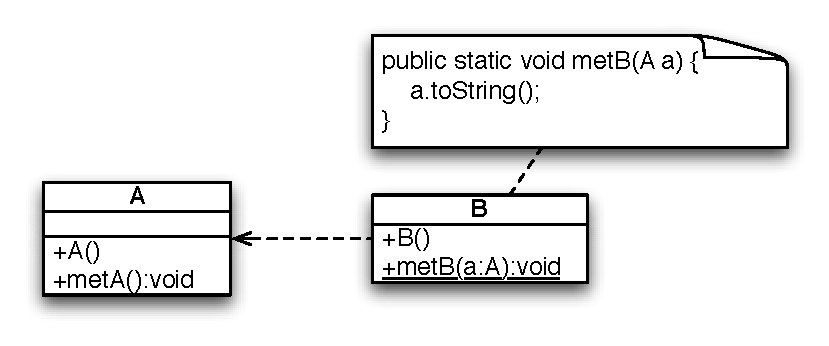
\includegraphics{fig/figure.pdf}}
\caption{My example\label{fig:examplefigure}}
\end{figure}


\section{Organization}

This diploma thesis is structured as follows: In Chapter \ref{ch:1} we describe
\ldots